\myChapter{Implementation of SOA-EA}\label{chap:osgiliath}
\minitoc\mtcskip
\vfill
\lettrine{I}{n} Chapter \ref{chap:soaea} we presented the services that conform an Evolutionary Algorithm and the process to design a service oriented EA. Although the previous examples can be developed using any SOA technology, this chapter presents OSGiLiath ({\em OSGi Laboratory for Implementation and Testing of metaHeuristics}), an implementation of SOA-EA based in OSGi. 

\section{Framework description}
This proposed environment is a  framework for the development of heuristic optimization applications, not centered on a concrete paradigm, and whose main objective is to promote the OSGi and SOA usage and offer to programmers the next features:

\begin{itemize}
\item Easy interfaces. After a study of the previous frameworks a complete interface hierachy has been developed.
\item Asynchronous data sending/receiving. Thanks to ECF distributed capabilities, the framework has easy distribution of services, without implementing specific source functions, like MPI or other distribution frameworks. Programmers do not need to write communication code. 
\item Component Oriented Programming. The framework is plug-in oriented, so new improvements can be added in easy way without modification of existent modules. Adding o modifying implementations of services can be performed without re-compilation of the source code.
\item Client/Server or Distributed Model. All components of the framework can communicate in a bi-directional way, so a central broker is not necessary if it is not required.
\item Paradigm independent. The framework is not focused in a type of metaheuristic.
\item Declarative Services. Bind interfaces to specific implementations can be done without modifying existent source code. Programmers do not need to instantiate implementations of the services.
\item Remote event handling: Using the OSGi advantages, users can use a powerful tool to synchronize or share data among services.
\end{itemize}

The source code is available at \url{http://www.osgiliath.org}, under a LGPL license.

\subsection{OSGiLiath organization}

By now, OSGiLiath counts with the next bundles:

\begin{itemize}
\item osgiliath: This is the core bundle. It includes all the interfaces common to the algorithms such as {\em Algorithm}, {\em AlgorithmParameters} or {\em Problem}. 
\item Evolutionary Algorithm:  Includes the {\em EvolutionaryAlgorithm} implementation and interfaces to create the rest of the services that form an EA: {\em Recombinator} and {\em Crossover}, {\em Mutator} and {\em Mutation}, {\em StopCriterion} or {\em FitnessCalculator}. It also provides interfaces for the creation of individuals: {\em Individual}, {\em Fitness}, {\em Gene}, and {\em Genome}. 
\item Basic Evolutionary Components: Includes several implementations (the most common ones) of the previous interfaces: {\em ListPopulation}, {\em ListIndividual}, {\em DoubleFitness}, {\em NGenerationStopCriterion}, {\em BasicOrderRecombinator}, {\em UPXListCrossover} and others.
\item Binary Problems: Includes implementation of well-known problems, such as OneMax and MMDP: {\em OneMaxFitnessCalculator}, {\em MMDPFitnessCalculator} or {\em BinaryProblemRandomInitializer}.
\item Function Problems: Multi-dimensional optimization functions, such as Griegwank or Rastrigin are implemented in this bundle, with their associate Initializers or Fitness Calculators.
\item NSGA2: Interfaces and implementations of services for the NSGA2 algorithm.
\item OSGiLiART: Service implementation for the creation of Evolutionary Art: {\em ArtisticIndividual} or {\em HistogramFitnessCalculator} are examples.
\item NoOSGi: Because OSGi allows the separation of source code with the OSGi framework capabilities, this bundle includes Java code to integrate the services without any specific technology (just using basic Object Oriented programming).
\item IntelligentManager: An example of how the services can be bound/unbound in real-time. By now, in each step the {\em IntelligentRandomManager} selects randomly from the available Crossovers, Mutators and Replacers implementations.
\end{itemize}

\section{Reasons to use OSGi}
OSGi has been selected for the development of this service oriented architecture instead Web Services  attending the following reasons:

\begin{itemize}

\item OSGi is faster, because it was designed for
  lightweight devices \cite{LimGateway08}. Therefore, it can be
  used in embedded devices, like Evolutionary Robotics
  \cite{Garcia2012testing}. On the contrary, Web services were created to integrate complex
  data interchange among different companies.  
\item The transmission protocol in web services is SOAP, which implies
  the transmission of an XML ({\em eXtension Markup
    Language}) file \cite{XML}. This file is usually too large (for example, a
  complete list of workers in a company). 
 EAs often need to send
  minimal information, but a large number of times (for example, the
  fitness of several individuals), so a complex transmission protocol
  is not recommended. OSGi includes a lot of mechanisms for data
  transmission, allowing more flexibility depending on the execution environment of
  the algorithms (for example, in a machine, in a local
  network, over the Internet, or even in more lightweight devices). 

 \item Unlike web services, OSGi includes a blackboard event-manager,
   that is, services inform what they are doing without indicating 
 any receiver. Other services can filter this information and actuate
 accordingly, so the synchronization is easier. For example, it is not
 mandatory to create a variable to count the number of times that the
 {\em Fitness Calculator} service is executed: an external service can track this number. 
 \item Due to the separation between OSGi and the source code of the
   services, the code of OSGi-based applications can be used in other
   Java-based applications without OSGi. For the same reason,
   frameworks written in Java can be migrated into services in a easy
   way, because no specific code is required to combine code from different programs. 
 \item Finally, OSGi includes other features that, although not related to SOA, facilitate the service development: version and package
   control, security and life-cycle management of the used
   components, that can be useful in the development of EAs 
   (as explained by \person{Wagner \etal} \cite{WagnerPlugins07}). These advantages can be used by the EA developers if
   they work in a team collaboration. 
\end{itemize}

More information about the application of OSGi in other areas, with good practices, benefices and lessons learned are provided by the authors in \cite{GarciaSanchez2013Gateway}.

The objective of this implementation is to promote SOA benefits and offer  these features to programmers:


\begin{itemize}
\item Well defined interfaces. As previously stated, service interfaces must be as abstract as possible.
\item Asynchronous data sending/receiving. Due to the distribution capabilities offered by OSGi, the presented implementation allows the direct distribution of services, without the need to implement specific functions in the source code, like MPI or other distribution mechanisms. EAs developers can use the existing distribution services or create new ones, if they want.
\item Service oriented programming. New improvements can be added without modifying the existing modules, that is, adding or modifying only the affected service implementations without modifying the source code of the other services.
\item Server/client or distributed model. All the components of this implementation can communicate in a bi-directional way, so it is not mandatory to use a central server to manage other nodes.
\item Paradigm independent. Although the first developments are focused on EAs, this architecture can be extensible to other kind of metaheuristics.
\item Remote event handling. Users can handle a
  powerful synchronization tool among distributed services using OSGi features. 
                               
\end{itemize}

The source code of OSGiLiath is available in \url{http://www.osgiliath.org} under a GNU/GPL license. This code is an updated version of the work published in \cite{GarciaSanchezDistributed2010}. 

 
\section{Service development in OSGiLiath}

Users have to define three elements to add a new service in OSGiLiath:


\begin{itemize}
\item {\em Service interface}. It is a Java interface. The user just needs to specify the operations that the service will perform.
\item {\em Service implementation}. The programmer just writes the code of the interface methods.
\item {\em Service description}. It is an XML file that indicates which
  interface is being implemented and which other services needs to be
  activated. 
\end{itemize}
These concepts were explained in detail in Chapter \ref{chap:soa}.
The presented implementation includes the interfaces defined in Chapter \ref{chap:soaea}, such as {\em Algorithm}, {\em StopCriterion}, {\em Population} or {\em Recombinator}. These interfaces are grouped with another interfaces that do not need to be a service. For example, the interface of the object {\em Individual}. This interface is used in the {\em Recombinator} interface, which receives a list of {\em Individual} objects to be recombined, and returns another list with the recombined ones.
Also, several implementations are included, like {\em EvolutionaryAlgorithm} (implementing {\em  Algorithm}) or the rest of  services explained in previous chapters, like the services for NSGA-II.


The source code of the method that executes the algorithm in the class {\em EvolutionaryAlgorithm} (implementation) is shown in Figure \ref{fig:javaevo}. It also includes methods to bind the six references to the service implementations that are needed: Population ({\em pop} in the code), StopCriterion, ParentSelector, Recombinator, Mutator, and Replacer. 


\newsavebox{\mintedbox}
\begin{lrbox}{\mintedbox}
\begin{minipage}{10cm}
\begin{minted}[mathescape,
               linenos,
               frame=lines,
               framesep=2mm]{java}
//References to the implementations to use
Population pop;
ParentSelector parentSelector;
Recombinator recombinator;
Mutator mutator;
Replacer replacer;

//Example of the method to obtain an implementation
//of the ParentSelector interface 
//(one function per reference)
void setParentSelector(ParentSelector sel){
  this.parentSelector = sel;
  //now sel is a reference to an implementation 
        //of ParentSelector
}

//Implementation of the start() method of the 
//Algorithm interface
public void start(){
  pop.initializePopulation();
  actualIteration = 0;
  do{
    //SELECT parents
    List<Individual> parents = 
    parentSelector.select(pop);
      
    //RECOMBINE parents
    List<Individual> offspring = 
    recombinator.recombine(parents);
      
    //MUTATE offspring
    List mutatedOffspring = 
    mutator.mutate(offspring);
      
    //SELECT new population. 
    //pop is modified here
    replacer.select(pop, parents, 
    offspring, mutatedOffspring);
      
    actualIteration++;
      
  }while(!stopCriterion.hasFinished());
    
}
\end{minted}
\end{minipage}
\end{lrbox}


\begin{SCfigure}[20][htb]
\usebox{\mintedbox}
\caption{Java code of the class {\em Evolutionary Algorithm}. This class implements the {\em Algorithm} interface, which defines the operation {\em start()} } 
\label{fig:javaevo} 
\end{SCfigure}


This is the code needed by every EA, so it not necessary to modify it (for example, to change from a GA to an ES).  The {\em Service Description} appears when the service interfaces are bound to execute the service implementation. Each implementation of a service has an XML file indicating which interface is being implemented, and also other properties. This file is used by OSGi to automatically bind the services. The service descriptor of the EA is shown in Figure \ref{fig:ds}. This file describes that the {\em EvolutionaryAlgorithm} class is an implementation of the {\em Algorithm} interface, and that it needs implementations of the interfaces {\em Population}, {\em Mutator}, {\em ParentSelector}, {\em Replacer}, {\em StopCriterion} and {\em Recombinator} to be activated.

It should be noted that this file usually can be modified using a friendly GUI, or from an assistant in Java IDEs, such as NetBeans or Eclipse (so, users do not have to care about its XML structure). The user interface to create this file in Eclipse is shown in Figure \ref{fig:xmlgui}. The interface being implemented is set in the lower part ({\em Algorithm}). The necessary services to activate this implementation are indicated in the upper part (with the cardinality and functions to set and unset the service implementations in the implementation source code).

\newsavebox{\mintedboxDS}
\begin{lrbox}{\mintedboxDS}
\begin{minipage}{10cm}
\begin{minted}[linenos,
               fontsize=\scriptsize,
               frame=lines,
               framesep=2mm]{xml}
<?xml version="1.0" encoding="UTF-8"?>
<scr:component xmlns:scr="http://www.osgi.org/xmlns/scr/v1.1.0" enabled="false"
immediate="true" name="OsgiliathEvolutionary" >
<implementation class="es.ugr.osgiliath.evolutionary.EvolutionaryAlgorithm"/>
<service>
<provide interface="es.ugr.osgiliath.algorithms.Algorithm"/>
</service>
<reference bind="setPopulation" cardinality="1..1"
interface="es.ugr.osgiliath.evolutionary.elements.Population"
name="Population" policy="static" unbind="unsetPopulation"/>
<reference bind="setMutator" cardinality="1..1"
interface="es.ugr.osgiliath.evolutionary.elements.Mutator"
name="Mutator" policy="static" unbind="unsetMutator"/>
<reference bind="setParentSelector" cardinality="1..1"
interface="es.ugr.osgiliath.evolutionary.elements.ParentSelector"
name="ParentSelector" policy="static" target="(selectorName=nsga2)" 
unbind="unsetParentSelector"/>
<reference bind="setReplacer" cardinality="1..1"
interface="es.ugr.osgiliath.evolutionary.elements.Replacer"
name="Replacer" policy="static" target="(replacerName=nsga2)" 
unbind="unsetReplacer"/>
<reference bind="setStopCriterion" cardinality="1..1"
interface="es.ugr.osgiliath.evolutionary.elements.StopCriterion"
name="StopCriterion" policy="static" unbind="unsetStopCriterion"/>
<reference bind="setRecombinator" cardinality="1..1"
interface="es.ugr.osgiliath.evolutionary.elements.Recombinator"
name="Recombinator" policy="static" unbind="unsetRecombinator"/>
<property name="algorithmName" type="String" value="EvolutionaryAlgorithm"/>
</scr:component>
\end{minted}
\end{minipage}
\end{lrbox}

\begin{SCfigure}[20][htb]
\usebox{\mintedboxDS}
\caption{Service descriptor of the Evolutionary Algorithm implementation.  Figure \ref{fig:xmlgui} shows the friendly user interface to automatically create  this file using the Eclipse program} 
\label{fig:ds} 
\end{SCfigure}

\begin{SCfigure}
\centering
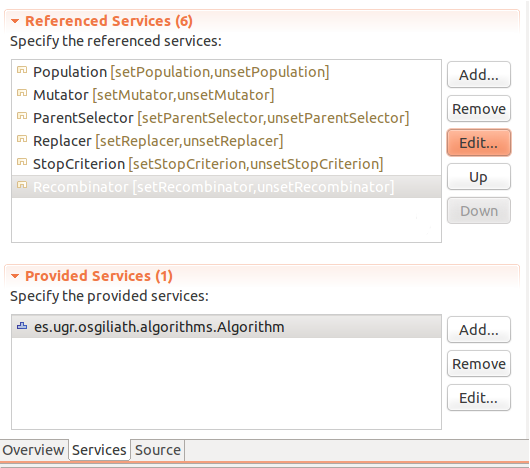
\includegraphics[width=8cm]{gfx/osgiliath/eclipse.png}

\caption{Graphic user interface in Eclipse that generates the Service Descriptor of Figure \ref{fig:ds} }.
\label{fig:xmlgui}
\end{SCfigure}

This XML file is read by the OSGi execution environment, which is the responsible to bind the available services to this implementation. For example, if a {\em ParentSelector} is activated, automatically is bound to the variable {\em parentSelector} through the function {\em setParentSelector}. The {\em cardinality} is also set in the file, in this case, only one implementation is necessary (not multiple). This file can be modified in execution time, so it is not required to re-compile the Java code to use and set new services.

In brief, each implementation of a service (\textit{$<$im\-ple\-men\-ta\-tion$>$}) indicates the interface to being implemented (\textit{$<$pro\-vi\-de in\-ter\-fa\-ce$>$}), and the other services this implementation needs (\textit{$<$re\-fe\-ren\-ce$>$}). 

Moreover, each service can provide properties to be used by other services to obtain more information and filtering. For example, in this case only the {\em Replacers} whose property {\em replacerName=nsga2} are used.


\subsection{Managing services: implementing the NSGA-II from the canonical GA}

Following the development example showed in Section \ref{sec:nsga2}, some extra services have been developed to convert the basic GA into a NSGA-II (and have also been added to OSGiLiath to be available for users).

There exist many options for the EA to pick up the appropriate service. The first of them is modifying the source code of the implementations. Obviously this is not recommended, because the service would not be loose coupled due to the specific OSGi code, and this is not a good SOA practice. The following ways makes the service usage not code-dependent:


\begin{itemize}
\item De-activating the implementation {\em Binary Tournament} from the OSGi administration console, and activating the implementation {\em Crowding Distance Selector} (that is, manually). This technique is not recommended, because all services are then managed by hand, and this is very difficult with a large number of services. However, the OSGi console allows modifying services in execution time, so it can be used in some cases (for example, to stop the service in a machine while another big task is being executed, and activate it again when this task is over).
\item Modifying the Service Descriptor of the {\em Evolutionary Algorithm} implementation to filter the desired implementations (for example, the attribute {\em target\-=``(selectorName\-=nsga2)''} in Figure \ref{fig:ds}). This option is used when the algorithm is fixed and does not need to be modified in execution time, and the number of operators and types are known in advance. However, as previously stated, new services can be added in execution time (for example, if the cardinality is set to multiple).
\item Using an external service that activates or de-activates desired implementations or modify their status. This technique must be used when self-adaptation properties are used in the algorithm, and it is presented in next subsections. 
\end{itemize}


None of these options needs to modify the source code of the existing services: they just indicates which services uses each time.

\subsection{Adding distributed capabilities}

As previously stated in Section \ref{sec:distribution}, one of the main advantages in SOA-EA is that services can be distributed, so the proposed implementation of the architecture  should also allow  the distribution and load balancing of the EA. In OSGiLiath all services can be distributed using the OSGi features. In this case, the distribution is performed using the service descriptor to set which service is distributable and which is the distribution technology that provides service discovering and data transmission.

OSGi allows several implementations for the service distribution. ECF\footnote{\url{http://www.eclipse.org/ecf/}} has been chosen because it is the most mature and accepted implementation (claimed by \person{Petzold \etal} \cite{petzold2011dynamic}), and it also supports the largest number of transmission protocols, including both synchronous and asynchronous communication. ECF also separates the source code from the discovery and transmission mechanism, allowing users to apply the most adequate technology to their needs, and providing the integration with existing applications. For example, the lines of Figure \ref{fig:remote} have been added to the service descriptor of {\em MOP2 Fitness Calculator} to distribute it in the local network.




\newsavebox{\mintedboxServer}
\begin{lrbox}{\mintedboxServer}
\begin{minipage}{10cm}
\begin{minted}[linenos,
               fontsize=\scriptsize,
               frame=lines,
               framesep=2mm]{xml}

<property name="service.exported.interfaces" type="String" value="*"/>
<property name="service.exported.configs" type="String" 
value="ecf.generic.server"/>
<property name="ecf.exported.containerfactoryargs" type="String" 
value="ecftcp://localhost:3787/server"/>
\end{minted}
\end{minipage}
\end{lrbox}

\begin{SCfigure}[20][htb]
\usebox{\mintedboxServer}
\caption{Lines added to the service descriptor of Figure \ref{fig:ds} to be discovered by other services in a network  (this can also be done in the GUI)} 
\label{fig:remote} 
\end{SCfigure}

In this case, it is only necessary to set the properties that ECF uses to identify the services being distributed in the network, indicating that all implemented interfaces are distributable (\texttt{ser\-vi\-ce\-.ex\-por\-ted\-.in\-ter\-fa\-ces}). Also, the communication technology to be used is established (\texttt{ecf\-.ge\-ne\-ric\-.ser\-ver}, although another kind of protocol could be used), and finally, the service URL (\texttt{ ecf\-.ex\-por\-ted\-.con\-tai\-ner\-fac\-to\-ry\-args}). As previously stated, the service properties can be modified from other services, so this properties can be added outside the XML. It should be noted that the source code of the services has not been modified to distribute them (as would happen if MPI had been used to perform the distribution, for example).




\subsection{Converting a basic algorithm into a self-adaptive one}

Previous sections remarked that the SOA-EA benefits are also related to self-adaptation. A simple example is presented here to demonstrate how easy is to convert a basic evolutionary algorithm into a self-adaptive one in OSGiliath. In this example, an intelligent service manages all the available operators. In this case, the service {\em IntelligentRandomManager} implements the interfaces {\em Parent Selector, Recombinator, Mutator} and {\em Replacer}. All operator implementations previously presented are added to the Manager in execution time (see Figure \ref{INTELLIGENTALGORITHM}) when they become activated in the system. Every time the EA calls an operator, this simple manager chooses randomly one of the available implementations it controls. To create this manager no code has to be modified. The manager also does not need specific code to acquire all operators in execution time: it is done automatically thanks to OSGi. As the rest of services, these operators can be activated in execution time and added to the manager. 



\subsection{Increasing interoperability with other systems}

As previously stated, another advantage of SOA is the programming language independence respect to the service interfaces. Although OSGi is a kind of SOA, it does not include  the capability of interoperability with other kind of services by default. However, adaptation services can be added to transform OSGi interfaces into other SOA interfaces, such as Web Services (presented in Chapter \ref{chap:soa}). So, services that are not written in Java, neither OSGi-based, could use services implemented in OSGiLiath (and vice-versa).

ECF includes a number of protocols for service discovery and service providers:
\begin{itemize}
\item Service Discovery API: Includes protocols to announce and discover remote services: Zeroconf, SLP/RFC 2608, Zookeeper, file-based and others \footnote{\url{http://wiki.eclipse.org/ECF_API_Docs\#Discovery_API}}.
\item Remote Service API: Includes protocols to establish the communication (data streams, formats and others): R-OSGi, ActiveMQ/JMS, REST, SOAP, XMPP, ECF Generic \footnote{\url{http://wiki.eclipse.org/ECF_API_Docs\#Remote_Services_API}}. This allow to communicate to systems that do not use OSGi or Java.
\end{itemize}

For example, using ECF all OSGi service interfaces could be transformed into WSDL interfaces automatically. Thus, these services could be used from other systems, that do not need to know the implementation language of the services in OSGiLiath. An example where an OSGi interface is transformed into a WSDL interface is shown in Figure \ref{AXISFIGURE}. The computation node A, based on OSGi, uses the OSGi interface of the computation node C to calculate the fitness. Node B uses the WSDL interface to do the same task. It is not necessary to modify existing services source code to convert an OSGi interface into a WSDL interface. This transformation is bi-directional: given an WSDL interface, it can also be transformed into a service to use inside OSGi. For example, the algorithms in GridUFO framework (presented in Chapter \ref{chap:distributedEAs}) could be used from OSGiLiath.






\begin{SCfigure}[20][htb]
\centering
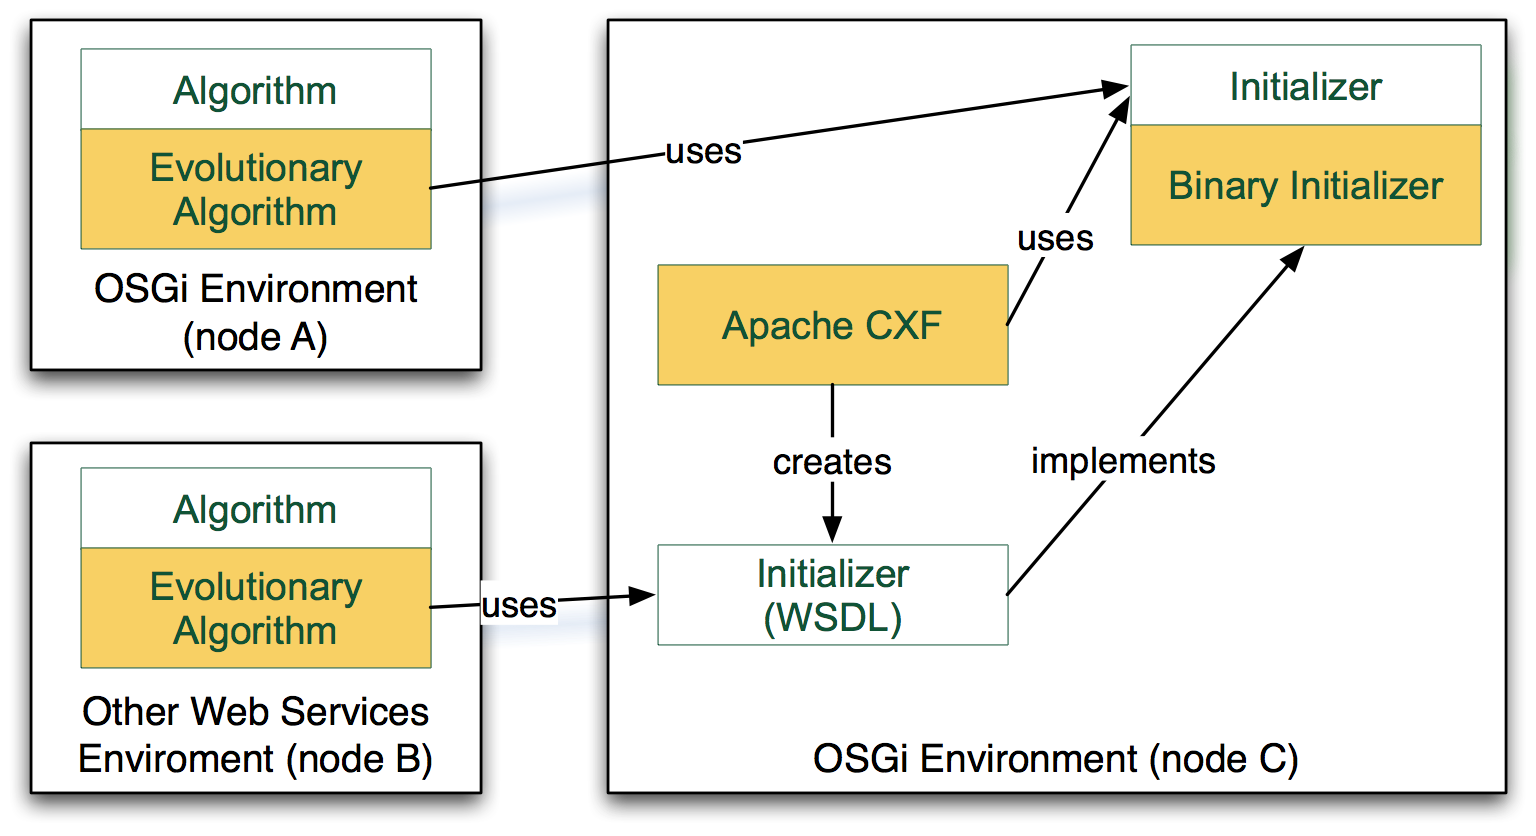
\includegraphics[width=10cm]{gfx/osgiliath/axis.png}


\caption{Communication with other kind of services. ECF service automatically creates WSDL interfaces for the OSGi interfaces to be used from other environments}
\label{AXISFIGURE}
\end{SCfigure}

\section{Experiments}
One may think that working with services usually implies an overhead. This is true when communication protocols like SOAP are used, because the transmitted XML must be generated and parsed. However, as SOA is independent of the implementations, services also can behave as normal method calls in the same machine.


The first experiment of this section is focused on this issue, and will demonstrate that the use of a SOA oriented implementation of an EA doesn't have to affect the execution time of the algorithm. To carry out this experiment, the Java source code of OSGiLiath has been run outside of the OSGi framework, and a normal Java class has been used to integrate the interfaces and implementations ``as is''. The population has been set to 64 individuals, parents have been selected using Binary Tournament, and the mutation rate has been fixed to 0.1. Worst individuals (parents and off-spring combined) are replaced, and the stop criterion has been set to 200 generations. Each experiment has been launched 30 times to solve the OneMax problem \cite{SchafferOnemax91}.



Since the OSGi framework adds features to the implementation of the algorithm that are similar (and even superior) to those offered by several of the frameworks described in Chapter \ref{chap:distributedEAs}, the same algorithm (with the same operators and parameters) has been coded using several well known frameworks, such as Mallba (C++), Algorithm::Evolutionary (Perl), and ECJ (Java). Table \ref{tab:times} shows the execution time achieved, average solution, and Lines of Code (LoC) needed to integrate the algorithm for each framework. All the algorithm implementations have been executed on the same computer, an Ubuntu 12.04 Linux Machine with Intel Core2 Quad CPU Q8200 @ 2.33GHz, 4 GB RAM, without any distribution mechanisms. The LoC have been calculated using {\em sloccount} program.






\begin{SCtable}[][t]
\resizebox{11cm}{!}{
\begin{tabular}{llll}
\hline
\rowcolor{colorCorporativoSuave}Name    &  Average solution    & Average Time (s)  & LoC \\
\hline\hline
\rowcolor{colorCorporativoMasSuave}OSGiLiath               &   612.36 $\pm$ 6.05  & 0.19 $\pm$ 18.21 &  10\\
\rowcolor{colorCorporativoSuave}OSGiLiath (without OSGi)&   613.36  $\pm$ 4.50 & 0.19 $\pm$ 22.74 &  103\\
\rowcolor{colorCorporativoMasSuave}MALLBA                  &   578.76 $\pm$ 7.48  & 0.16 $\pm$ 0.0003 &  2073\\
\rowcolor{colorCorporativoSuave}ECJ                     &   602.76 $\pm$ 6.08   & 1.40 $\pm$ 0.03 &  5\\
\rowcolor{colorCorporativoMasSuave}Algorithm::Evolutionary &   617.60 $\pm$ 12.92  & 7.78 $\pm$ 0.29 &  41\\
\hline
\end{tabular}
}
\caption{Comparison of tested EA frameworks in time and development.}
\label{tab:times}
\end{SCtable}

Results show that time of services of OSGiLiath is not affected by the OSGi framework: times are almost identical to the integration with Java code. Note that, although are services developed under SOA, and bound in runtime, they are not distributed. Algorithmically, all frameworks behaves the same, and results are not quite different. The differences among frameworks are produced because the different implementations of random generators, operators or logs, for example. In the work of \person{Merelo \etal} \cite{PERL}, these different behaviours are also justified.



Regarding LoCs, MALLBA has the higher number: this is because every algorithm is created as a ``skeleton'' and a duplication of code exist for each algorithm and problem to execute. This is produced because many operations affect global variables: for example the method {\em select\_offsprings()} affects the global variables {\em parents} or {\em aux}. Using this method as an external service would require a whole change in many parts of the code. Thanks the loose-coupling of Perl, many lines of code are saved using Algorithm::Evolutionary, mainly because many parameters and operators are defined by default.



ECJ and OSGiLiath do not require code to combine different operators, only modify configuration files without re-compilation. The difference is in ECJ the available operators must be known prior to execution (the interfaces are linked in the source code), while in OSGiLiath, all interfaces are bound in configuration files, or even without them (for example, appearing in the same network/machine). But there also exist limitations, because ECJ only provides a fixed ways of distribution mechanisms, and only certain parts of the framework can be accessed remotely, while in OSGiLiath all operators have the chance to be distributed if desired, modifying the configuration files.


It must be remarked that OSGiLiath does not try to compete with the other frameworks (they are widely accepted, completed and tested), it is only an example of how to develop EAs under the SOA paradigm.